\documentclass[sigconf]{acmart}

\AtBeginDocument{%
  \providecommand\BibTeX{{%
    \normalfont B\kern-0.5em{\scshape i\kern-0.25em b}\kern-0.8em\TeX}}}

\usepackage{dblfloatfix}
\usepackage{mathtools}
\usepackage{hyperref}
\usepackage[htt]{hyphenat}
\usepackage{listings}
\usepackage{xcolor}
\usepackage[framemethod=tikz]{mdframed}
\usepackage{algorithm}
\usepackage{algpseudocode}
\usepackage{float}
\usepackage{caption}
\usepackage{tikz}
\usepackage{subcaption}
\usepackage{graphicx}
\usepackage{csvsimple}
\usetikzlibrary{shapes,arrows,arrows.meta}

\definecolor{codegreen}{rgb}{0,0.6,0}
\definecolor{codegray}{rgb}{0.5,0.5,0.5}
\definecolor{codepurple}{rgb}{0.58,0,0.82}
\definecolor{backcolour}{rgb}{0.95,0.95,0.92}

\lstdefinestyle{mystyle}{
	backgroundcolor=\color{backcolour},
	commentstyle=\color{codegreen},
	keywordstyle=\color{magenta},
	numberstyle=\tiny\color{codegray},
	stringstyle=\color{codepurple},
	basicstyle=\ttfamily\footnotesize,
	breakatwhitespace=false,
	breaklines=true,
	captionpos=b,
	keepspaces=true,
	numbers=left,
	numbersep=5pt,
	showspaces=false,
	showstringspaces=false,
	showtabs=false,
	tabsize=2,
}

\lstset{style=mystyle}

\begin{document}

\title{Enhancement of images with uneven illumination}
\subtitle{Enhancing images with uneven illumination using ensemble learning\\Group ID: \#1}

% AUTHORS:
\author{Til Mohr}
\affiliation{}
\email{tv.mohr@stud.uis.no}

\author{Alexander Mühleisen}
\affiliation{}
\email{alexandermuhleisen@gmail.com}

% DATE:
\date{\today}



\begin{abstract}
This paper introduces a method for enhancing images with uneven illumination by leveraging the strengths of ensemble learning. Uneven illumination in images can severely affect the performance of computer vision algorithms and the visual quality for human observers. Our approach combines three classical image enhancement techniques: Unsharp Masking, Retinex, and Homomorphic Filtering, to address different aspects of the problem. These techniques are integrated through an ensemble learning framework that employs a fusion network of perceptrons for each color channel. The proposed method is unique in its application of ensemble learning to this specific problem of image enhancement. The results demonstrate that the method can effectively improve the visibility of details in images and can serve as a robust preprocessing step for further image analysis tasks.
\end{abstract}

\keywords{image processing, image enhancement, uneven illumination, ensemble learning}

%% Remove copyright footer
\settopmatter{printacmref=false}
\setcopyright{none}
\renewcommand\footnotetextcopyrightpermission[1]{}
\pagestyle{plain}
%% ------------------------

%%
%% This command processes the author and affiliation and title
%% information and builds the first part of the formatted document.
\maketitle


\section{Introduction}\label{sec:intro}
Image enhancement is a critical preprocessing step in computer vision that improves the visual quality of images, particularly when they suffer from uneven illumination. Uneven illumination can result from various factors such as lighting variances and camera limitations, leading to shadows, glares, and inconsistent brightness levels. Such issues pose significant challenges in downstream tasks like object recognition, segmentation, and tracking, as these algorithms rely heavily on uniform illumination to extract features accurately.

The goal of image enhancement in this context is to compensate for these illumination variances without introducing artifacts or losing important details. Traditional techniques like Unsharp Masking, Retinex, and Homomorphic Filtering address this issue from different angles. However, they can fall short when faced with complex illumination patterns or when one technique's strengths could complement another's weaknesses.

To bridge this gap, we propose a simple ensemble learning-based image enhancement framework that combines the strengths of individual enhancement methods. Ensemble learning, typically used in machine learning for decision-making tasks, can be effectively applied to image processing. By integrating the outputs of different enhancement techniques, we hope to produce a single, high-quality image that benefits from the cumulative strengths of each method. A main research goal of this report is to investigate to which extent the different enhancement methods contribute to the final result, and in which situations the fused image is superior to the individual images produced by the enhancement methods.

The rest of the paper is structured as follows. Section \ref{sec:theory} reviews the current enhancement methods and their theoretical underpinnings. In Section \ref{sec:method} we detail our ensemble learning approach and the training of the fusion network. We then present our experimental results in Section \ref{sec:results}, followed by a discussion of their implications in Section \ref{sec:discussion}. Finally, we conclude with a summary of our findings and suggestions for future work.

\section{Theory}\label{sec:theory}
In this section we will dive into different methods to enhance images with uneven illumination. We will start with a brief introduction to the problem and then discuss different methods to solve it, as well as how to evaluate the results.

\subsection{Problem description}\label{sec:problem}
Uneven illumination refers to the irregular distribution of light intensity across an image. In essence, it disrupts the uniformity of the visual output, leading to disparities in brightness and contrast, often observable as glares or shadows. These disparities can mask essential features and details, making the subject of the image less identifiable. This becomes especially problematic when images need to be processed further for various computer vision tasks. In fields like optical microscopy, for example, consistent illumination is crucial for accurately identifying and segmenting microscopic entities. Uneven lighting can obscure crucial cellular structures or make similar-looking entities appear distinct, hampering accurate analysis \cite{dey2019uneven}.

To counter this issue, the goal is to enhance the image in a manner that simulates its capture under uniform illumination conditions. By doing so, we aim to restore a natural appearance to the image, preserving details and minimizing artifacts introduced by uneven lighting. This correction enables better analysis, ensuring that conclusions drawn are based on the actual subject and not on lighting imperfections \cite{dey2019uneven}.

\subsection{Unsharp Masking}\label{sec:unsharp}
Unsharp masking is a technique to sharpen images, enhancing edges and fine details by utilizing a blurred copy of the image. The technique's somewhat paradoxical name comes from how it operates: by subtracting the blurred version from the original image, it isolates the 'unsharp' or high-frequency parts—the details and edges—then these are amplified and recombined with the original, resulting in a clearer, more defined image. The process can be expressed mathematically as \cite{shi2021unsharp,morishita1988unsharp,deng2010generalized}:
\begin{equation}
g(x,y) = f(x,y) + \lambda \cdot (f(x,y) - Blur(f)(x,y))
\end{equation}
Here, $f(x,y)$ represents the original image, $Blur(f)(x,y)$ is the blurred version of the original image, and $\lambda$ is a positive value determining how much sharpening is applied. The blurring is often achieved with a Gaussian filter, a common choice for such image processing tasks \cite{shi2021unsharp,morishita1988unsharp,deng2010generalized}. An implementation of the unsharp masking algorithm is shown in Listing \ref{lst:unsharp}.

\subsection{Retinex}\label{sec:retinex}
Retinex theory forms the basis of a research area aimed at replicating human vision perception through models. This field has birthed various algorithms to improve the visual quality of images. Notably, the Multi-Scale Retinex with Chromacity Preservation (MSRCP) algorithm has been developed. MSRCP enhances the original Multi-Scale Retinex (MSR), which itself is an advancement of the Single Scale Retinex (SSR). The SSR is described by the following mathematical expression \cite{petro2014multiscale,barnard1998investigations}:
\begin{equation}
\text{R}{n_i}(x,y) = \log(f_i(x,y)) - \log(f_i(x,y) \ast F_n(x,y))
\end{equation}
In this formula, $f_i(x,y)$ represents the pixel intensity of the input image at location $(x,y)$ in the $i$-th color channel, while $F_c(x,y)$ is a Gaussian function used to analyze the surrounding pixels with a standard deviation of $\sigma = n$. Building upon SSR, MSR averages the SSR outputs over multiple scales, as indicated here \cite{petro2014multiscale,barnard1998investigations}:
\begin{equation}
\text{R}{MSR_i}(x,y) = \sum_{n=1}^{N} \omega_n \cdot \text{R}_{n_i}(x,y)
\end{equation}
where $\omega_n$ are the weights for each scale. Research has indicated that while MSR can enhance image details, it may also lead to desaturated colors. Hence, MSRCP was introduced. This method first creates an improved image using MSR and then adjusts this image's colors to span the entire available color range \cite{petro2014multiscale}. Afterward, it combines the color-stretched image with the original to adjust and intensify the original image's colors \cite{petro2014multiscale}. An example of how this is implemented can be found in Listing \ref{lst:retinex}.

\subsection{Homomorphic Filtering}\label{sec:homomorphic}
The intensity of an image at pixel $(x,y)$ can be described as the product of the illumination $i(x,y)$ and the reflectance $r(x,y)$ \cite{voicu1997practical,fan2011homomorphic}:
\begin{equation}
	f(x,y) = i(x,y) \cdot r(x,y)
\end{equation}
In the frequency domain, illumination changes across the image are typically manifested by low frequencies, while high frequencies are associated with reflectance changes. Therefore, by applying the logarithm to the image, one can separate the illumination and reflectance components of the image \cite{voicu1997practical,fan2011homomorphic}:
\begin{equation}
	\log(f(x,y)) = \log(i(x,y)) + \log(r(x,y))
\end{equation}
Applying the Fourier transform to this log-image, a filter $H(u,v)$ can be applied to attenuate the low frequencies, that is the frequencies responsible for illumination changes, and increasing the high frequencies responsible for detail. To finish the enhancement, we revert the process by applying an inverse Fourier transform and exponentiation  \cite{voicu1997practical,fan2011homomorphic}:
\begin{equation}
	f(x,y) = \exp(\mathcal{F}^{-1}(\mathcal{F}(\log(f(x,y))) \cdot H(u,v)))
\end{equation}
This process is illustrated in Figure \ref{fig:homomorphic-pipeline}.

\begin{figure}
	\centering
	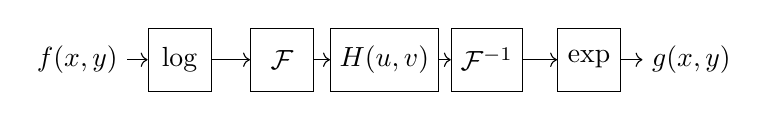
\begin{tikzpicture}[node distance=1.3cm, auto]
		% Define the style for the operation nodes
		\tikzstyle{operation}=[rectangle, draw=black, minimum size=0.8cm, text centered]

		% Define nodes
		\node (input) {$f(x,y)$};
		\node (op1) [operation, right of=input] {$\log$};
		\node (op2) [operation, right of=op1] {$\mathcal{F}$};
		\node (op3) [operation, right of=op2] {$H(u,v)$};
		\node (op4) [operation, right of=op3] {$\mathcal{F}^{-1}$};
		\node (op5) [operation, right of=op4] {$\exp$};
		\node (output) [right of=op5] {$g(x,y)$};

		% Define edges
		\draw[->] (input) -- (op1);
		\draw[->] (op1) -- (op2);
		\draw[->] (op2) -- (op3);
		\draw[->] (op3) -- (op4);
		\draw[->] (op4) -- (op5);
		\draw[->] (op5) -- (output);
	\end{tikzpicture}
	\captionof{figure}{Homomorphic filtering pipeline.}
	\label{fig:homomorphic-pipeline}
\end{figure}

There are numerous types of linear filters that can be applied; Voicu et al. suggest using a Butterworth filter of the second order \cite{voicu1997practical}. This particular filter focuses on reducing the impact of low frequencies while accentuating high frequencies:
\begin{align}
	H(u, v) = H'(\rho) = \gamma_1  - \gamma_2 \cdot \frac{1}{1 + 2.415 \cdot \left(\frac{\rho}{\rho_c}\right)^{4}},\\
	\text{where} \qquad \rho = \sqrt{u^2 + v^2}
\end{align}
Here, $\gamma_1$ and $\gamma_2$ are constants that can be adjusted for the desired outcome, with $\gamma_1 \approx \gamma_H$ and $\gamma_2 \approx \gamma_H - \gamma_L$, and $\rho_c$ is the cutoff frequency \cite{voicu1997practical}. The filter's general shape is depicted in Figure \ref{fig:homomorphic-filter}.

\begin{figure}
	\centering
	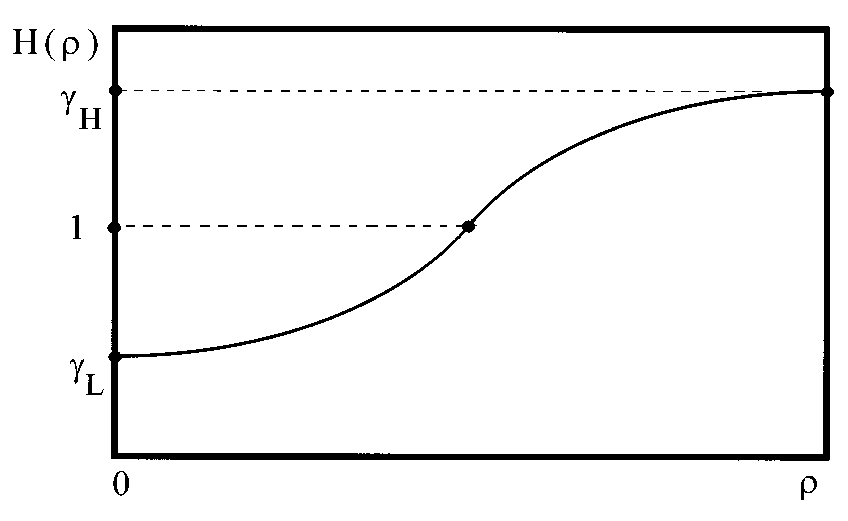
\includegraphics[width=0.45\textwidth]{images/filter.png}
	\captionof{figure}{General form of the filter used in homomorphic filtering \cite{voicu1997practical}.}
	\label{fig:homomorphic-filter}
\end{figure}

Additionally, Fan et al. recommend including a step for histogram equalization after the filtering to further improve the image's contrast \cite{fan2011homomorphic}. For color images, the homomorphic filtering process can be applied to each individual color channel,  e.g. the illumination channel of HSI images, or to every channel as in RGB images \cite{voicu1997practical,fan2011homomorphic}. An example of how to implement this approach is provided in Listing \ref{lst:homomorphic}.

\subsection{Assessment of Image Enhancement}\label{sec:evaluation}
Determining the success of image enhancement depends on the purpose of the process. For aesthetic purposes, a simple visual check may be enough to judge improvement. If the enhancement serves as preparation for a subsequent task like image segmentation, its success should be measured based on how it improves the results of that task. Nevertheless, there are specific objective criteria we can use to evaluate enhancement:

\subsubsection{RMS Contrast}\label{sec:rms-contrast}
Contrast refers to how distinctly the dark and light areas of an image stand apart, essentially how easy it is to distinguish different objects in the picture. When correcting an image with inconsistent lighting, our goal is to better the contrast in regions that were initially similarly lit. Thus, the enhancement may not always boost the overall contrast but could lead to local improvements. RMS contrast is calculated as the standard deviation of pixel intensities across the entire image \cite{dey2019uneven}:
\begin{equation}
\text{RMS Contrast} = \sqrt{\frac{1}{N \cdot M} \sum_{i=1}^{N} \sum_{j=1}^{M} (I(i,j) - \bar{I})^2}
\end{equation}

\subsubsection{Discrete Entropy}\label{sec:discrete-entropy}
Entropy describes the amount of information in an image, where a high entropy means that the image contains a lot of information, and a low entropy means that the image contains little information, i.e. a flat image has zero entropy. Enhancing an image with uneven illumination should increase the amount of information in the image, and therefore increase the entropy. The discrete entropy is defined as \cite{dey2019uneven,ye2007discrete}:
\begin{equation}
	\text{Discrete Entropy} = - \sum_{i} P_i \cdot \log_2(P_i)
\end{equation}
where $P_i$ is the probability that the difference between two adjacent pixels is $i$.

\section{Methodology}\label{sec:method}
This paper aims to investigate the efficacy of combining Unsharp Masking (UM), Retinex (RTX), and Homomorphic Filtering (HF) enhancement techniques into a coherent ensemble framework. We propose a approach by integrating these methods through a fusion network, comprising three distinct perceptron networks corresponding to each color channel. This section delineates the methodology in detail, including the structure of the fusion network and the training of its parameters.

\subsection{Fusion Network}\label{sec:fusion}
Our exploration centers on a fusion network that amalgamates the strengths of UM, RTX, and HF, detailed in Sections \ref{sec:unsharp}, \ref{sec:retinex}, and \ref{sec:homomorphic}, respectively. The operational sequence of our model begins with generating intermediate enhanced images through each method, denoted as $g_{UM}$, $g_{RTX}$, and $g_{HF}$. Subsequently, these images are inputted into the fusion network to yield the final enhanced image $g_{F}$.

\begin{algorithm}
	\caption{Fusion Network}\label{alg:fusion}
	\begin{algorithmic}
	\Require $g_{UM}$, $g_{RTX}$, $g_{HF}$ in HSI color space
	\Require $w_{c} \in \mathbb{R}^3$ for $c \in \{hsi\}$
	\Ensure $N \coloneqq \text{width}(g_{UM}) = \text{width}(g_{RTX}) = \text{width}(g_{HF})$
	\Ensure $M \coloneqq \text{height}(g_{UM}) = \text{height}(g_{RTX}) = \text{height}(g_{HF})$
	\State $g_{F} \gets 0^{N \times M \times 3}$
	\For{$c \in \{hsi\}$}
		\For{$(x,y) \in \{1, \dots, N\} \times \{1, \dots, M\}$}
			\State $g_{F}(x,y,c) \gets w_{c_1} \cdot g_{UM}(x,y,c)$
			\State \qquad \qquad \qquad  $+ w_{c_2} \cdot g_{RTX}(x,y,c)$
			\State \qquad \qquad \qquad $+ w_{c_3} \cdot g_{HF}(x,y,c)$
		\EndFor
	\EndFor
	\State \Return $g_{F}$
	\end{algorithmic}
	\end{algorithm}

The fusion network is constructed from three individual perceptron networks, each tailored for a specific channel of the HSI color space. For any given pixel at coordinates $(x,y)$, each perceptron receives three inputs: the values of channel $c \in {hsi}$ from $g_{UM}$, $g_{RTX}$, and $g_{HF}$. The output is the channel $c$ of the pixel $(x,y)$ in $g_{F}$. The fusion process is algorithmically represented in Algorithm \ref{alg:fusion}. The weights $w_{c} \in \mathbb{R}^3$, for each channel $c \in {hsi}$, are parameters that determine the influence of each intermediate image and are optimized during the training process, as discussed in Section \ref{sec:training}. In our experiments, the use of bias was omitted. The fusion process is visually summarized in Figure \ref{fig:fusion-pipeline}.

\begin{figure}
	\centering
	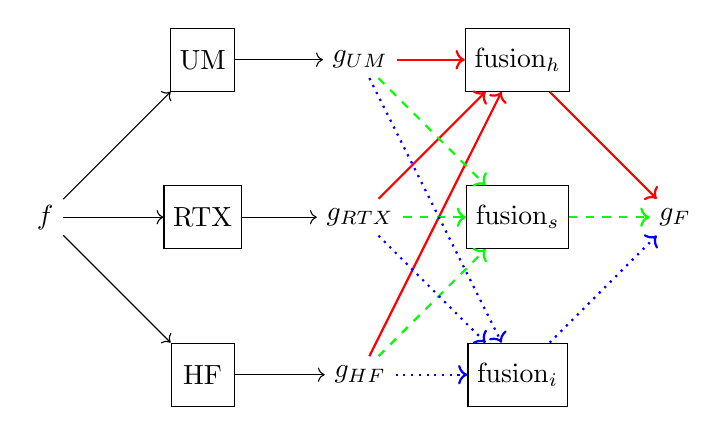
\begin{tikzpicture}[node distance=2cm, auto]
		% Define the style for the operation nodes
		\tikzstyle{operation}=[rectangle, draw=black, minimum size=0.8cm, text centered]

		% Define nodes
		\node (input) {$f$};
		\node (RTX) [operation, right of=input] {RTX};
		\node (UM) [operation, above of=RTX] {UM};
		\node (HF) [operation, below of=RTX] {HF};
		\node (g_UM) [right of=UM] {$g_{UM}$};
		\node (g_RTX) [right of=RTX] {$g_{RTX}$};
		\node (g_HF) [right of=HF] {$g_{HF}$};
		\node (H) [operation, right of=g_UM] {$\text{fusion}_h$};
		\node (S) [operation, right of=g_RTX] {$\text{fusion}_s$};
		\node (I) [operation, right of=g_HF] {$\text{fusion}_i$};
		\node (output) [right of=S] {$g_F$};

		% Define edges
		\draw[->] (input) -- (UM);
		\draw[->] (input) -- (RTX);
		\draw[->] (input) -- (HF);

		\draw[->] (UM) -- (g_UM);
		\draw[->] (RTX) -- (g_RTX);
		\draw[->] (HF) -- (g_HF);

		\draw[red,thick,arrows = {->}] (g_UM) -- (H);
		\draw[red,thick,arrows = {->}] (g_RTX) -- (H);
		\draw[red,thick,arrows = {->}] (g_HF) -- (H);
		\draw[green,thick,arrows = {->}, dashed] (g_UM) -- (S);
		\draw[green,thick,arrows = {->}, dashed] (g_RTX) -- (S);
		\draw[green,thick,arrows = {->}, dashed] (g_HF) -- (S);
		\draw[blue,thick,arrows = {->}, dotted] (g_UM) -- (I);
		\draw[blue,thick,arrows = {->}, dotted] (g_RTX) -- (I);
		\draw[blue,thick,arrows = {->}, dotted] (g_HF) -- (I);

		\draw[red,thick,arrows = {->}] (H) -- (output);
		\draw[green,thick,arrows = {->}, dashed] (S) -- (output);
		\draw[blue,thick,arrows = {->}, dotted] (I) -- (output);
	\end{tikzpicture}
	\captionof{figure}{Pipeline of the fusion network approach. Red solid arrows symbolize the fusion of the hue channel, green dashed arrows symbolize the fusion of the saturation channel, and blue dotted arrows symbolize the fusion of the intensity channel.}
	\label{fig:fusion-pipeline}
\end{figure}

\subsection{Implementation}\label{sec:implementation}
For the implementation of our fusion network, we employed the \texttt{PyTorch} machine learning framework. It involves three distinct linear fully connected layers, one for each color channel. An abridged version of the code for the fusion network is presented in Listing \ref{lst:fusion}. Comprehensive explanations of the theoretical underpinnings and implementations for UM, RTX, and HF are provided in Sections \ref{sec:unsharp}, \ref{sec:retinex}, and \ref{sec:homomorphic}, with corresponding code snippets in Listings \ref{lst:unsharp}, \ref{lst:retinex}, and \ref{lst:homomorphic}. The entire codebase is made accessible on GitHub\footnote{URL: \url{https://github.com/CodingTil/eiuie}}.

\begin{mdframed}[backgroundcolor=backcolour,leftmargin=0cm,hidealllines=true,innerleftmargin=0cm,innerrightmargin=0cm,innertopmargin=0cm,innerbottommargin=-0.65cm]
\lstinputlisting[language=Python, caption=Fusion Model,label=lst:fusion]{listings/fusion.py}
\end{mdframed}

\subsection{Training}\label{sec:training}
The training of the weight parameters $w_{c} \in \mathbb{R}^3$ for each channel $c \in {hsi}$ is imperative for effective image enhancement. Leveraging the perceptron networks, the weights are refined through supervised learning. In an optimal setting, our training dataset comprises images with uneven illumination and their evenly illuminated counterparts. However, no such dataset is known to us. Due to the absence of a directly relevant dataset, we adapted the LOL-dataset, which includes image pairs with low and normal exposure \cite{wei2018deep}.

The training process involved using both the low-light and normal-light images from each pair as input, with the normal-light images always serving as the target output. This dual-input strategy was intended to calibrate the model to enhance underexposed areas without exaggerating well-lit sections.

With a dataset size of approximately $2.4$ billion samples (pixels), we were limited by memory constraints to utilize only half of this dataset. We adopted the Adam optimizer with a learning rate of $0.001$ and a batch size of $2^{15}$. The training was set to run for $1000$ epochs, but early stopping criteria were met shortly after the $100$th epoch. Remarkably, the entire training process was completed in about 10 minutes on a single NVIDIA L4 Tensor Core GPU.

\section{Results}\label{sec:results}
In this section, we conduct a comparative analysis of three image enhancement approaches: \textit{Unsharp Masking} (UM), \textit{Retinex} (RTX), \textit{Homomorphic Filtering} (HF), and our proposed fusion model (F). To asses the qualitiy of image enhancement we use visual inspection as well as the utilization of objective metrics such as RMS contrast and discrete entropy. We evaluated our methods using a dataset consisting of ten images.

Figure \ref{fig:visual_comparison_hike3} presents a visual comparison between the three different enhancement methods and our fusion model. The selected example image showcases a dimly illuminated stonewall in the foreground contrasted against a brightly lit landscape in the background. Notably, the original image lacks the clarity to distinguish the separate stones in the wall due to low contrast. All methods, except for unsharp masking, succeed in enhancing the quality of the dimly illuminated part of the image. This enhancement is evident as the individual stones of the wall become visible. Homomorphic filtering performs worse than Fusion and Retinex in this scenario, as it introduces unwanted artifacts in the enhanced dimly illuminated section of the image.
One major challengs for enhancment methods is to preserve the color of the original image. Unsharp masking performs best in this context, whereas HF results in a green tint in the image, especially in the previously dimly illuminated areas. Both Retinex and our fusion model cause the colors to fade. Besides of the color shift HF, RTX and our fusion model introduce noise to the image. 


\begin{figure*}
    \subfloat[\centering Original]{{\includegraphics[width=0.45\textwidth]{images/hike_3_O.jpg} }}%
    \qquad
    \subfloat[\centering Fusion]{{\includegraphics[width=0.45\textwidth]{images/hike_3_F.jpg} }}%
	\subfloat[\centering Unsharp masking]{{\includegraphics[width=0.45\textwidth]{images/hike_3_UM.jpg} }}%
    \qquad
    \subfloat[\centering Retinex]{{\includegraphics[width=0.45\textwidth]{images/hike_3_RTX.jpg} }}%
	\subfloat[\centering Homomorphic Filtering]{{\includegraphics[width=0.45\textwidth]{images/hike_3_HF.jpg} }}% 
	\qquad
    \caption{visual comparison of enhanced images}
    \label{fig:visual_comparison_hike3}
\end{figure*}


\begin{table}[]
	\begin{tabular}{l|lllll}
	 	             & \textbf{O}      & \textbf{F}     & \textbf{UM }    & \textbf{RTX} & \textbf{HF} \\
	\textbf{Example 1}       &		  &                &       & \\
	RMS contrast     & 319.57 & 120.11 & 366.01 & 180.75 & 213.33 \\
	d. entropy       & 5.14   & 6.27 & 5.16   & 6.75  & 6.04\\		 
    \hline
	\textbf{Average} (10 s)   &		  &                &       & \\
	RMS contrast     & 111.00 & 67.12 & 124.91 & 87.71 & 139.92 \\
	d. entropy       & 3.98   & 4.71  & 4.35   & 4.70  & 4.79\\
	 
	\end{tabular}
	\caption{comparison of Enhancement via RMS contrast and density}
	\label{tab:image_enhancement_measure}
\end{table}

 
Table \ref{tab:image_enhancement_measure} presents a comparision of the different methods concerning RMS contrast and discrete density. The average values are based on a sample size of 10 different images. Among the methods, unsharp masking and homomorphic filtering demonstrate the most significant improvement in RMS contrast, while our fusion model performs least effectively. Regarding discrete density, Retinex, Homomorphic Filtering and our fusion model show similar performance, while unsharp masking performs the poorest.
To interpret the varying performance results depending on the measure it is essential to understand what each measure represents. The RMS contrast contains information about the pixel variance of the entire images. Consequently, an increase in contrast within specific areas of an image contributes to an overall increase in RMS contrast measure. Discrete density measures the quantity of information encapsulated within the images. As observed in the visual comparision unsharp masking manage to improve the contrast in already well-illuminated areas of the image. However, it falls short in improving the poorly illuminated segments, leaving them relatively unchanged. Consequently, unsharp image fails to reveal information from the under-illuminated parts. This explains why unsharp masking shows good performance in improving rms contrast but shows significant weaker performance regarding to discrete density.
The fusion modell significantly increase the discrete density while concurrently reducing the RMS contrast. This observation aligns with our visual assessment, where the fusion model effectively enhanced the details in poorly illuminated areas, bringing out previously hidden information. However, this improvement came at the cost of a reduction in color vibrancy, consequently diminishing the overall contrast in the image which leads to a decrease in rms contrast.

\begin{table}
	\begin{tabular}{l|lll}
					& UM 	& RTX 		& HF     \\
		Hue 	  	& 0.0994	& 0.2782	& 0.5596  \\
		Saturation 	& 0.1376	& -0.0597	& 0.3378  \\
		Intensity  	& 0.0032	& 0.3836	& 0.4488  \\
		
	\end{tabular}
	\caption{wheigts for each chanel}
	\label{tab:weights}
\end{table}

Table \ref{tab:weights} shows the weights associated to each method for each channel within the fusion model. The weights attributed to the unsharp masking method  are relatively low across all channels, indicating a minor contribution to the fusion model. Conversely, the Homomorphic Filtering method exhibits the highest weights across all channels, signifying its substantial role within the fusion model. Note that the  weight for the saturation chanel of the Retinex method is negative. This indicates that the saturation chanel of the Retinex method is substracted in the fusion model. 



\section{Discussion}\label{sec:discussion}
In this section we discuss the implications of our proposed fusion model. 

The visual comparison demonstrates that each enhancement method exhibits strengths and weaknesses. Unsharp Masking is particularly proficient in preserving color information and increasing contrast in already well-illuminated areas but was less effective in enhancing poorly illuminated parts of the image. Retinex and Homomorphic Filtering show noticeable improvements in dimly illuminated sections, enhancing the visibility of finer details but at the expense of color preservation. However, Homomorphic Filtering introduces unwanted artifacts, especially in the enhanced dimly illuminated areas.
The idea behind our fusion model is to combine the strengths of each method, resulting in a more balanced enhancement. The results of our experiments demonstrate that the fusion model effectively enhances the details in poorly illuminated areas without introducing unwanted artifacts like Homomorphic filtering. However, concerning color vibrancy, the fusion model lags behind the other methods. This is noticeable in the visual comparison as well as in the results of the objective metrics. The fusion model significantly increases the discrete density while concurrently reducing the RMS contrast. This observation aligns with our visual assessment, where the fusion model effectively enhanced the details in poorly illuminated areas, revealing hidden information at the cost of faded colors.

The weights of the fusion model (table \ref{tab:weights}) indicate that the unsharp masking method plays a minor role within the fusion model. This is in line with our visual assessment, where the unsharp masking method was the least effective in enhancing the details in poorly illuminated areas. The Homomorphic Filtering method exhibits the highest weights across all channels, signifying its substantial role within the fusion model. This is also in line with our visual assessment, where the Homomorphic Filtering method was the most effective in enhancing the details in poorly illuminated areas. However the fusion model manage to outperform the Homomorphic Filtering regarding to enhancing poorly illuminated areas while concurrently reducing the unwanted artifacts introduced by the Homomorphic Filtering method.

Regarding to color vibrancy and overall contrast our fusion model performance significant worse than the other methdos. This might be due to the fact that the fusion model is trained on a dataset consisting of images with low and normal exposure. Consequently, the fusion model is calibrated to enhance underexposed areas without exaggerating well-lit sections. This calibration is not optimal for enhancing images with uneven illumination. Therefore, the fusion model is not able to enhance the well-lit sections of the image as effectively as the other methods. This is also reflected in the weights of the fusion model (table \ref{tab:weights}), where the weights of the unsharp masking method are relatively low across all channels.

\section{Conclusion}\label{sec:conclusion}

The goal of this paper was to investigate the efficacy of combining Unsharp Masking (UM), Retinex (RTX), and Homomorphic Filtering (HF) enhancement techniques into a coherent ensemble framework. We proposed a approach by integrating these methods through a fusion network, comprising three distinct perceptron networks corresponding to each color channel. The weights of the fusion network are trained using a dataset consisting of images with low and normal exposure. 
The results of our experiments demonstrate that the fusion model effectively enhances the details in poorly illuminated areas without introducing unwanted artifacts like Homomorphic filtering. However, concerning color vibrancy, the fusion model lags behind the other methods. This is noticeable in the visual comparison as well as in the results of the objective metrics. The fusion model significantly increases the discrete density while concurrently reducing the RMS contrast. This observation aligns with our visual assessment, where the fusion model effectively enhanced the details in poorly illuminated areas, revealing hidden information at the cost of faded colors.






%%
%% If your work has an appendix, this is the place to put it.


%%
%% The next two lines define the bibliography style to be used, and
%% the bibliography file.
\bibliographystyle{ACM-Reference-Format}
\bibliography{main}

\newpage
\appendix

\section{Listings}
\subsection{Unsharp Masking}\label{sec:unsharp-listing}
\begin{mdframed}[backgroundcolor=backcolour,leftmargin=0cm,hidealllines=true,innerleftmargin=0cm,innerrightmargin=0cm,innertopmargin=0cm,innerbottommargin=-0.65cm]
\lstinputlisting[language=Python, caption=Unsharp masking,label=lst:unsharp]{listings/unsharp_masking.py}
\end{mdframed}

\subsection{Homomorphic Filtering}\label{sec:homomorphic-listing}
\begin{mdframed}[backgroundcolor=backcolour,leftmargin=0cm,hidealllines=true,innerleftmargin=0cm,innerrightmargin=0cm,innertopmargin=0cm,innerbottommargin=-0.65cm]
\lstinputlisting[language=Python, caption=Homomorphic filtering, label=lst:homomorphic]{listings/homomorphic_filtering.py}
\end{mdframed}

\subsection{Retinex}\label{sec:retinex-listing}
\begin{mdframed}[backgroundcolor=backcolour,leftmargin=0cm,hidealllines=true,innerleftmargin=0cm,innerrightmargin=0cm,innertopmargin=0cm,innerbottommargin=-0.65cm]
\lstinputlisting[language=Python, caption=Retinex,label=lst:retinex]{listings/retinex.py}
\end{mdframed}

\end{document}
\endinput
